\documentclass[12pt]{book}

\usepackage[a4paper,outer=1.4in,inner=0.8in,vmargin=3cm]{geometry}

\usepackage{natbib}
\usepackage{graphicx}
\usepackage{amsthm}
\usepackage{amsmath}
\usepackage{setspace}
\usepackage{color}
\usepackage{lmodern}

\usepackage{sidecap}
\usepackage[scaled]{helvet}
\usepackage{caption}


\setlength{\marginparwidth}{1in}

\newcounter{todos}
\newcounter{comments}
\newcounter{figcomments}
\newcounter{advisorcomments}
\newcounter{questions}

\setcounter{tocdepth}{4}

\definecolor{grey}{rgb}{0.4,0.4,0.4}
\definecolor{brown}{rgb}{0.5,0.0,0.0}
\definecolor{orange}{rgb}{0.7,0.3,0.}
\DeclareCaptionFont{grey}{\color{grey}}
\captionsetup{margin=10pt,font=small,labelfont=bf,format=plain,textfont=grey,labelfont=grey}

\renewcommand*\familydefault{\sfdefault} %% Only if the base font of the document is to be sans serif
\usepackage[T1]{fontenc}
\linespread{1.2}

\title{Demonstrating Quantum Speed-Up with a Two-Transmon Quantum Processor.}
\author{Andreas Dewes}

\theoremstyle{definition}
\newtheorem{theorem}{Theorem}[chapter]
\newtheorem{axiom}{Axiom}[theorem]

\newcommand{\bracket}[1]{\left< #1 \right>} % for Dirac brackets
\newcommand{\ket}[1]{\left| #1 \right>} % for Dirac bras
\newcommand{\bra}[1]{\left< #1 \right|} % for Dirac kets
\newcommand{\todo}[1]{
  \addtocounter{todos}{1}
	\textcolor{red}{!\arabic{todos}!}
	\marginpar{
		\begin{spacing}{0.5}
			\textcolor{red}
				{
				{\flushleft \scriptsize  \linespread{0.8} To Do \arabic{todos}: #1}
				}
		\end{spacing}
	}
}
\newcommand{\figcomment}[1]{
	%To do: Fix the bug that makes the counter value increase by 2 each time this command is called.
	\addtocounter{figcomments}{1}
	\textcolor{orange}{Figure Comment \arabic{figcomments}: #1}
}

\newcommand{\comment}[1]{
  \addtocounter{comments}{1}
	\textcolor{orange}{!\arabic{comments}!}
	\marginpar{
		\begin{spacing}{0.5}
			\textcolor{orange}
				{
				{\flushleft \scriptsize  \linespread{0.8} Comment \arabic{comments}: #1}
				}
		\end{spacing}
	}
}

\newcommand{\question}[1]{
  \addtocounter{questions}{1}
	\textcolor{blue}{?\arabic{questions}?}
	\marginpar{
		\begin{spacing}{0.5}
			\textcolor{blue}
				{
				{\flushleft \scriptsize  \linespread{0.8} Question \arabic{questions}: #1}
				}
		\end{spacing}
	}
}

\newcommand{\advisorcomment}[1]{
  \addtocounter{advisorcomments}{1}
	\textcolor{yellow}{!\arabic{advisorcomments}!}
	\marginpar{
		\begin{spacing}{0.5}
			\textcolor{yellow}
				{
				{\flushleft \scriptsize  \linespread{0.8} Advisor comment \arabic{advisorcomments}: #1}
				}
		\end{spacing}
	}
}

\begin{document}

\maketitle

\tableofcontents

\listoffigures

\listoftables

\chapter{Introduction}

%-General introduction in the research field: Quantum mechanics, superposition, entanglement

\section{Quantum Computing}

%-Discuss the interest of quantum computation and possible paradigms: Classical, surface-code, topological...

\section{Superconducting Quantum Bits}

%-Discuss types of superconducting quantum bits (flux, phase, charge, hybrid)

\section{Circuit Quantum Electrodynamics}

%-Discuss CQED as the architecture used throughout this work.


\chapter{Theoretical Foundations} \label{chapter:theory}

The design and realization of a superconducting qubit processor demands knowledge of many different techniques and technologies. In this chapter we therefore provide the reader with the most essential theoretical foundations that we will employ in the following chapters of this thesis book. We will begin our discussion with a general overview of classical and quantum information processing, followed by an introduction to superconducting quantum circuits. Afterwards, we will introduce the concept of circuit quantization and discuss the Cooper pair box, the Transmon qubit and circuit quantum electrodynamics. Finally we will give a short overview of the physics of Josephson bifurcation amplifiers.

\section{Classical \& Quantum Information Processing}

\begin{SCfigure}
	\includegraphics[width=8cm]{"./material/figures/introduction/bloch_sphere"}
	\caption{The Bloch sphere representation of a qubit state $\ket{\psi} = \cos{\frac{\theta}{2}}\ket{0}+e^{i\phi}\sin{\frac{\theta}{2}}\ket{1}$. The state $\ket{\psi}$ is fully characterized by specifying its ``latitude'' and ``azimuth'' angles $\theta$ and $\phi$. Pure quantum states will always lie on the surface of the Bloch sphere, whereas mixed quantum states can also lie anywhere inside the sphere.}
	\label{fig:BlochSphere}
\end{SCfigure}

By definition, computing designates the activity of using computer hardware and software to process information, or {\it data}. Classical information processing can be divided in so-called {\it analog and digital information processing}, the former being based on continously changeable physical quantities whereas the latter is based on incrementally changeable quantities. The fundamental unit of digital information processing is the so-called {\it bit}, which represents a boolean (true/false) information. The discipline of theoretical computer science has been created to investigate the fundamental limits and properties of classical information processing. One of the main foundational theorems of theoretical computer science is the so-called {\it Church-Turing thesis} which provides a universal computing model by saying (basically) that everything which is computable can be efficiently computed using a {\it Turing machine}. Such a Turing machine, in turn, is a simple theoretical device which is able to run programs that operate on a discrete set of data using a well-specified set of operations. The Turing machine is universal in the sense that any other classical computing device can be efficiently emulated using a Turing machine with the appropriate program and data.

\smallskip

In the early 1980, Richard Feynman discovered that a classical Turing machine as described above would be unable to efficiently simulate a quantum-mechanical system \citep{feynman_simulating_1982}. He introduced the concept of a {\it quantum Turing machine} that would be able to simulate quantum-mechanical systems in an efficient manner. A few years later, David Deutsch took up Feynman's idea and developed an information processing framework based on quantum mechanics \citep{deutsch_quantum_1985}, coining the terms {\it quantum computing} and {\it quantum information processing}. He showed that by making use of different properties of quantum mechanics one could solve certain mathematical problems faster than possible with any classical computer \citep{deutsch_quantum_1985}. The work by Deutsch created a large interest in the physics community and led to a huge theoretical and experimental effort aimed at realizing a working quantum computer and developing quantum algorithms that solve relevant real-world problems.

\section{Principles of Quantum Computing}

In this section we will discuss the basic principles of quantum computing, including quantum bits and quantum gates. We will also briefly dicsuss some examples of quantum algorithms that are relevant to this work. We will focus on the {\it quantum gate} approach to quantum computing since it is the method relevant to this work, ignoring other approaches such as {\it one-way quantum computing} \citep{raussendorf_one-way_2001}, {\it adiabatic quantum computing} \citep{farhi_quantum_2000} or {\it topological quantum computing} \citep{kitaev_fault-tolerant_2003}.

\subsection{Quantum Bits}

Similar to classical computing, in quantum computing one can define a fundamental unit of information, the so called {\it quantum bit} or {\it qubit}. Such a qubit is a quantum-mechanical two-level system described by the wavefunction
%
\begin{equation}
\ket{\psi} = \cos{\frac{\theta}{2}}\ket{0}+e^{i\phi}\sin{\frac{\theta}{2}}\ket{1}.
\end{equation}
%
As can be seen, the state of such a qubit can be described by a pair of real numbers $\theta$ and $\phi$ that characterize the occupation probability of each of the two basis states $\ket{0}$ and $\ket{1}$ and the phase between them. A useful and intuitive representation of such a single-qubit state is the so-called {\it Bloch sphere representation}, which is shown in fig. \ref{fig:BlochSphere}. In this representation, a pure state $\ket{\psi}$ is located on a unit sphere. The north and south poles of this sphere correspond to the qubit states $\ket{0}$ and $\ket{0}$. All states lying between those two correspond to superposition states, which are characterized by their ``latitude'' and ``azimuth'' angles $\theta$ and $\phi$. The Bloch sphere representation can be generalized for mixed single-qubit states, whose state vector will lie inside the Bloch sphere.

\subsection{Quantum Gates}

Analogously to classical information processing one defines {\it quantum gates} that act on individual or multiple qubits and allow us to process information with them. Such a quantum gate can be described as a unitary operator acting on a part of the Hilbert space representing the qubit register. Theoretically there is an infinite number of possible quantum gates, however in order to describe all possible quantum operations that can be performed on a qubit register of arbitrary length it is sufficient to defined a so-called {\it universal set of quantum gates}. Such a set contains a small number of quantum gates that can, by concatenation, produce any arbitrary unitary quantum operator, as shown by the so-called {\it Solovay-Kitaev theorem} \citep{nielsen_quantum_2000,dawson_solovay-kitaev_2005}. Such a universal gate set that will be especially relevant to this work consists of the three single-qubit rotation matrices
%
\begin{eqnarray}
   R_x(\theta)  & = & e^{-i\sigma_x\frac{\phi_x}{2}} \\ 
   R_y(\theta)  & = & e^{-i\sigma_y\frac{\phi_y}{2}} \\ 
   R_z(\theta)  & = & e^{-i\sigma_z\frac{\phi_z}{2}} 
\label{eq:universal_single_qubit_gates}
\end{eqnarray}
%
where $\sigma_x$, $\sigma_y$ and $\sigma_z$ are the three Pauli spin operators
%
\begin{align}
  \sigma_x  =  \left( \begin{array}{cc} 0 & 1 \\ 1 & 0 \end{array} \right) 
  & & \sigma_y  =  \left( \begin{array}{cc} 0 & -i \\ i  &  0\end{array} \right) 
  & & \sigma_z  =  \left( \begin{array}{cc} 1 & 0 \\ 0 & -1 \end{array} \right) 
\label{eq:pauli_operators}
\end{align}
%
togehter with the so-called $i\mathrm{SWAP}$ two-qubit operator, which has the representation
%
\begin{equation}
i\mathrm{SWAP} = \left( \begin{array}{cccc} 1 & 0 & 0 & 0 \\ 0 & 0 & i & 0 \\ 0 & i & 0 & 0 \\ 0 & 0 & 0 & 1  \end{array}  \right)
\end{equation}
%
in the basis $(\ket{00},\ket{01},\ket{10},\ket{11})$. In principle, two single-qubit gates with a fixed rotation angle (e.g. $R_x(\pi/4)$ and $R_y(\pi/4)$) would be sufficient to form a universal set of quantum gates \citep{dawson_solovay-kitaev_2005}, however it is often advantageous if one can use single-qubit rotations with arbitary rotation angles around all three axes of the Bloch sphere since it can significantly reduce the number of gates required to implement a desired unitary operator.

\subsection{Quantum Algorithms}

The interest in quantum computing is mainly due to the fact that certain problems can be solved faster on a quantum computer than on a classical computer. By faster we mean here that the order $\cal{O}$ of the runtime of the algorithm increases faster on a classical computer than on a quantum computer as a function of the problem size, i.e. the number of bits needed to encode the problem. Up to this day it has not been demonstrated that a quantum computer can perform all tasks faster than a classical computer. However, a small number of real-world problems have been found that can be solved exponentially to polynomially faster on a quantum computer. Here we cite only the two most ``famous'' ones:

\begin{enumerate}
\item \textbf{The Shor Factorization Algorithm} Developed by Peter Shor in 1994 \citep{shor_algorithms_1994,shor_polynomial-time_1995}, this algorithm can factorize a binary number of length $N$ into its prime factors in $\begin{mathcal}O\end{mathcal}(\log^3{N})$ steps, therefore exponentially outperforming any known classical factorization algorithm. There is large interest in this algorithm since products of large prime numbers are routinely used in asymmetric cryptography.
\item \textbf{The Grover Search Algorithm}: Discovered by Lev Grover in 1996 \citep{grover_fast_1996}, this search algorithm can find a single well-defined state in an unsorted database of size $N$ in $\begin{mathcal}O\end{mathcal}(\sqrt{N})$ steps, being hence quadratically faster than a classical search algorithm.
\end{enumerate}

\subsection{Quantum Simulation}

Another domain of interest for quantum computers is so called {\it quantum simulation}. Here the goal is to simulate the behaviour of an arbitrary quantum system using a quantum computer by either engineering the quantum computer in direct analogy with the system being modeled (so called {\it analog quantum simulation}) or by numerically simulating the Hamiltonian of the quantum system on a general-purpose quantum computer (so-called {\it digital quantum simulation}). Since no classical computer can simulate a quantum system efficiently, there is a large interest in quantum simulation, especially in the fields of biology and chemistry.

\subsection{Realization of a Quantum Computer}

To realize a working quantum computer it is necessary to implement highly coherent qubits that can be manipulated, read out and coupled with high fidelity. So far, no fully working quantum computer has been experimentially demonstrated. However, larger progress towards the realization of such a quantum computer has been achieved in the last decade. Promising approaches for the realization of a quantum computer include --among others-- ions trapped in magnetic and electric fields \citep{monroe_demonstration_1995,cirac_quantum_1995}, nuclear magnetic resonance of organic molecules \citep{jones_nmr_2001,vandersypen_experimental_2001}, cold atomic gases \citep{briegel_quantum_2000}, photonic circuits \citep{knill_scheme_2001}, semiconductor structures \citep{loss_quantum_1998} and, last but not least, superconducting structures. Since this work treats only superconducting qubits of the Transmon type we will focus our attention on them in the following sections. We will explain how we can realize a reliable qubit using superconducting structures and how we can implement circuits to manipulate, couple and read out the qubit state.

\section{Superconduting Quantum Circuits}

In this section we will discuss several types of superconducting circuit elements that are most relevant to this work. First, we will introduce the reader to the Josephson junction, which is the device we use to realize superconducting qubits and amplifiers. Afterwards, we discuss the properties of transmission lines and tranmission line resonators that we use extensively for implementing readout and coupling elements in our qubit design. Then, we present a general method for the quantization of arbitrary electrical circuits that we will use afterwards to perform canonical quantization of our circuits. We will use this method to derive the Hamiltonian of the Cooper pair box and treat the Transmon qubit as a special case. Then we will give a short overview of the field of circuit quantum electrodynamics and finally introduce the reader to the Josephson and cavity bifurcation amplifiers that we use for our qubit readout.

\subsection{The Josephson junction}

The core element used to construct quantum circuits is the so-called {\it Josephson junction}, being equivalent in significance to the transitor in classical circuits. A Josephson junction is based on a disovery of Brian Josephson, which published a now-classical paper on quantum tunneling between weakly coupled superconductors \citep{josephson_possible_1962}. He found, that such a {\it weak link} between two superconductors could support a supercurrent $I$ described by the simple formula
%
\begin{equation}
I = I_c\sin{\varphi}
\end{equation}
%
where $\varphi = \varphi_2-\varphi_1$ and $\varphi_1$ and $\varphi_2$ are the gauge-invariant superconducting phases at each side of the link. $\varphi$ is related to the voltage between the electrodes of the Junction as
%
\begin{equation}
U = \frac{\Phi_0}{2\pi}\frac{\partial \varphi}{\partial t}
\end{equation}
%
where $\Phi_0 =h/2e \approx 2.05\times 10^{-15}$ is the so-called {\it magnetic flux quantum}. Thes two simple equations yield a system exhibiting a  wealth of interesting physical phenomena which are used today in various applications. The energy associated with the Josephson junction is given as
%
\begin{equation}
E = E_J(1-\cos{\varphi})
\end{equation}
%
where $E_J = I_c \Phi_0/2\pi$ is the so-called {\it Joesephson energy}. In addition to this Josephson energy, the junction usually has an energy associated to its capacitance (formed by its two seperated electrodes) given as $E_c = Q^2/2C$, with $Q$ being the charge difference between the electrodes of the junction.

\smallskip

For currents $I\ll I_c$, the Josephson junction behaves approximatively like a nonlinear inductance with
%
\begin{equation}
L_J(\varphi) = \frac{\Phi_0}{2\pi I_c \cos{\varphi}} \approx L_{J0}\left[1+\frac{\varphi^2}{2}+\begin{mathcal}O\end{mathcal}(\varphi^4)\right]\label{eq:josephson_inductance}
\end{equation}
%
, where $L_{J0}=\Phi_0/2\pi I_c$. Later we will show how to make use of these properties of the Josephson junction to construct a qubit and a qubit readout with it.

\subsection{Coplanar Waveguides And Resonators}

\begin{SCfigure}
	\includegraphics[width=6cm]{"./material/figures/introduction/transmission_lines"}
	\caption{a) The circuit diagram of a grounded (coaxial) tranmission line. b) The circuit diagram of a grounded coplanar waveguide (CPW) tranmission line.}
	\label{fig:tline_schematic}
\end{SCfigure}

Another circuit element that we will encounter many times in this work is the so-called {\it coplanar waveguide} (CPW), which we will use later to e.g. realize on-chip microwave resonators. A coplanar waveguide can be treated in a more general way as a {\it transmission line}. In principle, such a transmission line is a structure with a large extension in one direction that is capable of transmitting electromagnetic waves along its extended dimension. The circuit symbol that we will use in this work for a transmission line is shown in fig. \ref{fig:tline_schematic}a. A coplanar waveguide is a flat structure with a central conductor that is seperated by a gap from a groundplane on either side, as shown in fig. \ref{fig:tline_schematic}b. A detailed treatment of the physics of tranmission lines can be found e.g. in \cite{pozar_microwave_2011}. For this introduction we will skip this basic treatment and start directly with the equation that describes the propagation of an electromagnetic wave along the extended dimension $z$ of the waveguide, which is
%
\begin{eqnarray}
V(z,t) & = & \exp{\left(i\omega t\right)}\cdot\left(V^+ \exp{\left(-i\gamma z\right)}+V^-\exp{\left(i\gamma z\right)}\right) \\
I(z,t) & = & \frac{1}{Z_0}\exp{\left(i\omega t\right)}\cdot\left(V^+ \exp{\left(-i\gamma z\right)}-V^-\exp{\left(i\gamma z\right)}\right)
\end{eqnarray}
%
Here, $\gamma = \alpha+i\beta = \sqrt{(R+i\omega L)(G+i\omega C)}$ is the so-called {\it propagation constant} which describes the dispersion and damping of electromagnetic waves along the waveguide and $\omega$ the circular frequency of the electromagnetic wave. The voltages $V^+$ and $V^-$ correspond to waves traveling in different directions along the waveguide.

\smallskip

If we regard now a waveguide of finite length $l$, we can model the voltages and currents at both ends of it as \citep{pozar_microwave_2011}
%
\begin{equation}
\left( \begin{array}{c} V_1 \\ I_1 \end{array}\right) = \left( 
		\begin{array}{cc}
			\cos{\gamma l} & iZ_r \cos{\gamma l} \\
			i Y_r \sin{\gamma l} & \cos{\gamma l}
		\end{array}
		\right) \cdot \left(
		\begin{array}{c}
			V_2 \\ I_2
		\end{array}
		\right), \label{eq:cpw_abcd_matrix}
\end{equation}
%
where $Z_R=\sqrt{\begin{mathcal}L/C\end{mathcal}}$ is the impedance of the waveguide and $Y_R=1/Z_R$ the corresponding admittance. In the next section we will make use of the equation above to calculate the transmission properties of an open-ended waveguide.

\subsection{Transmission Line Resonators}

One can easily create a resonator using a coplanar waveguide as described in the last section. Here, we will discuss the open-ended $\lambda / 2$ CPW resonator used in our experiments to realize the qubit readout resonator. To create a resonator out of a CPW line, we terminate the line at one end by an open gap and connect the other end to a drive line through an input capacitance $C_g$. We make use of eq. (\ref{eq:cpw_abcd_matrix}) to calculate the end voltages and currents of the resonator,demanding that $I_2=0$ (since the resonator is open-ended). We obtain for the voltage $V_1$ and current $I_2$ the relation
%
\begin{eqnarray}
V_1 & = & \cos{\gamma l} V_2 \\
I_1 & = & i Y_r \sin{\gamma l} V_2
\end{eqnarray}
%
The impedance of the resonator is given as $V_1/I_1 = -i Z_R \cot{\gamma l}$. The input impedance of the resonator as seen through the gate capacitance $C_g$ is then
%
\begin{equation}
Z_{in} = -i Z_r \cot{\gamma l}-\frac{i}{\omega C_g} \label{eq:cpw_impedance}
\end{equation}
%
The $S_{11}$ reflection coefficient of the resonator when coupling it to an input line with impedance $Z_0$ is
%
\begin{equation}
S_{11} = \frac{Z_{in}-Z_0}{Z_{in}+Z_0} = \frac{i(Z_R\cot{\gamma l}+1/\omega C_g)-Z_0}{Z_0+i(Z_r\cot{\gamma l}-1/\omega C_g)}
\end{equation}
%
Now, when measuring the reflection of an incoming signal with voltage $V^+$ at frequency $f=2\pi \omega$ and phase $\phi_0$, the phase of the relected signal $\phi_{ref}$ will be simply given as $\phi_{ref}-\phi_0=\mathrm{Arg}[V^-/V^+] = \mathrm{Arg}[S_{11}]$. Fig \ref{fig:lambda_over_4_response} shows this phase along with the absolute value of the input impedance $|Z_{in}|$ for an exemplatory resonator, shown in reduced units of $[l/v]$, with impendances $Z_r=Z_0=50\;\mathrm{\Omega}$, $\alpha=0$ and $C_g=10^{-3}/\omega_0\;[\mathrm{Hz}\cdot \mathrm{F}]$, where $\omega_0 = 2\pi f_0$ is the angular resonance frequency of the resonator.

\begin{SCfigure}
	\includegraphics[width=10cm]{"./material/mathematica/cpw_lambda_over_4_phase_and_z"}
	\caption{The reflected phase and absolute value of the input impedance of a $\lambda/4$ resonator with $Z_r=Z_0=50\;\mathrm{\Omega}$, $\alpha=0$ and $C_g=10^{-3}/\omega_0\;[\mathrm{Hz}\cdot\mathrm{F}]$, plotted as a function of the reduced frequency.}
	\label{fig:lambda_over_4_response}
\end{SCfigure}

We can approximatively model the distributed CPW resonator as a lumped element $LC$ resonator, which is useful for e.g. calculating its quality factor. If we regard the input impedance of the resonator in the vicinity of $\omega_0$ such that $\Delta \omega = \omega -\omega_0 \ll \omega_0$ and $\beta l = \pi +\pi\Delta \omega /\omega_0$, we obtain an effective impedance
%
\begin{equation}
Z_{in} = -i\frac{Z_{r}}{(\Delta \omega \pi / \omega_0)}
\end{equation}
%
We can identify the quantities in this equation with the input impedance of a parallel LC-resonator, which is approximatively given as
%
\begin{equation}
Z_{in} = \frac{Z_0}{1+2i Q \Delta \omega / \omega_0}
\end{equation}
%
with $Q=\omega_0 RC$. This yields an effective inductance and capacitance for the transmission line resonator of
%
\begin{eqnarray}
L_{r} & = & \frac{1}{\omega_0^2 C} \\
C_{r} & = & \frac{\pi}{2\omega_0 Z_r}
\end{eqnarray}
%
When coupling this resonator to an input transmission line of impedance $Z_0$ through a  capacitance $C_g$ as before, the quality factor of the coupled (or {\it loaded}) resonator will be given as
%
\begin{equation}
Q_L = \omega_0^* \frac{C+C^*}{1/R_{r}+1/R^*}
\end{equation}
%
where we have introduced an effective resistance, capacitance and resonance frequency given as
%
\begin{eqnarray}
R^* & = & \frac{1+\omega_0^2 C_g^2 Z_0^2}{\omega_0^2 C_g^2 Z_0} \\
C^* & = & \frac{C_g}{1+\omega_0^2 C_g^2 Z_0^2} \\
\omega_0^* & = & \frac{1}{\sqrt{L_r(C_r+C_g)}}
\end{eqnarray}
%
We will make use of these relations and the fact that the external quality factor can be tuned by the value of the gate capacitance $C_g$ when designing the qubit readout resonator. In the next paragraph, we will introduce the concept of circuit quantization that we will later use to develop a quantum-mechanical description of the transmission line resonator discussed here.

\subsection{Quantization of Electrical Circuits}

In this section we will outline a general method to treat arbitary electrical circuits as the ones discussed before within the framework of quantum-mechanics, hence {\it quantizing} them. This introduction on circuit quantization presented in this chapter is based on an seminal article by M. Devoret \cite{devoret_quantum_1995}.

\begin{SCfigure}
	\includegraphics[width=5cm]{"./material/figures/introduction/sample_circuit"}
	\caption{An exemplatory superconducing circuit made of a Josephson junction, an inductor, a capacitor and a voltage source. The circuit topology can be described by two nodes (including ground) or three branches.}
	\label{fig:SampleCircuit}
\end{SCfigure}

Fig. \ref{fig:SampleCircuit} shows an exemplatory circuit made of an inductance, a capacitor, a Josephson junction and a voltage source. A circuit as this one is fully characterized by the parameters of its elements and its toplogy. The latter can be described -- following the laws of Kirchhoff -- as a set of nodes $j$ connected by a number of branches $i$ . In classical circuit theory, each branch is described by a voltage $V_i$ between its ends and a current $I_{i}$ flowing through it. The Kirchhoff laws demand that the sum of the branch voltages $V_i$ along any closed path must be zero. Equivalently one may demand that the sum of currents flowing in and out of each node must be zero. For the quantization of electrical circuits it is usually more convenient to replace voltages and currents with branch charges and fluxes that are defined as
%
\begin{eqnarray}
\Phi_i(t) & = & \int\limits_{-\infty}^t V_i(t') dt' \\
Q_i(t) & = & \int\limits_{-\infty}^t I_i(t') dt'
\end{eqnarray}
%
For these branch charges and fluxes we can define two Kirchoff laws
%
\begin{align}
\sum\limits_{i} Q_i  =  Q_c & & , & & \sum\limits_{i}\Phi_i = \Phi_c \label{eq:kirchhoff_charge}
\end{align}
%
where $Q_c$ and $\Phi_c$ are constants and where the first sum includes charges $Q_i$ of all elements connected to a certain node and the second one contains all fluxes $\Phi_i$ around a closed path of the circuit. To quantize such a circuit made up of non-dissipative elements we can follow the method given in \cite{yurke_quantum_1984}, writing the Lagrangian of the circuit as 
%
\begin{equation}
\begin{mathcal}L\end{mathcal} = \sum\limits_i \begin{mathcal}V\end{mathcal}_i - \sum\limits_i \begin{mathcal}T\end{mathcal}_i
\end{equation}
%
where $\begin{mathcal}V\end{mathcal}_i$ and $\begin{mathcal}T\end{mathcal}_i$ are the potential and kinetic energies associated to each circuit element. For a circuit composed entirely of capacitors and inductors, this Lagrangian is given as
%
\begin{equation}
\begin{mathcal}L\end{mathcal}(\Phi_1,\hdots,\Phi_n,\dot{\Phi}_1,\hdots,\dot{\Phi}_n) = \frac{1}{2}\sum\limits_i C_i \dot{\Phi}_i^2-\frac{1}{2}\sum\limits_i \frac{\Phi_i^2}{L_i} \label{eq:circuit_lagrangian}
\end{equation}
%
If needed, resistors can be described within the Lagrangian formalism by modeling them as transmission lines with a characteristic impedance matching their resistance \citep{yurke_quantum_1984}. We can also include general nonlinear capacitances and impedances that obey the relations $\dot{\Phi}=f_C(Q)$ and $\dot{Q}=g_L(\Phi)$ between their node flux and charge, whose energies are given as
%
\begin{eqnarray}
E_C = \int\limits_0^Q f_C(Q)dQ \\
E_L = \int\limits_0^\Phi g_L(\Phi)d\Phi
\end{eqnarray}
%
A Josephson junction, for example, can be described as a nonlinear inductance with $g_L^{JJ}(\Phi)=I_c\sin{(2\pi\Phi/\Phi_0)}$, having an associated energy
%
\begin{equation}
E_L^{JJ} = \int\limits_0^\Phi I_c\sin{\left(2\pi\Phi/\Phi_0\right)}=E_J(1-\cos{\left[2\pi\frac{\Phi}{\Phi_0}\right]}),
\end{equation}
%
where $E_J = I_c\Phi_0/2\pi$. Tranmission lines can be quantized by a similar approach, as shown e.g. in \citep{yurke_quantum_1984}. External charges and fluxes can be modeled as ``pre-charged'' capacitances and inductances that get renormalized at the end of the quantization process \citep{devoret_quantum_1995}. From the Lagrangian as given by eq. (\ref{eq:circuit_lagrangian}) we obtain then the equations of motion of the system by variation of the action
%
\begin{equation}
\frac{\partial}{\partial t}\left( \frac{\partial \begin{mathcal}L\end{mathcal}}{\partial\dot{\Phi}_i}\right)-\frac{\partial \begin{mathcal}L\end{mathcal}}{\partial \Phi_i} = 0
\end{equation}
%
Finally, by imposing the charge-conservation equations as given by eq. (\ref{eq:kirchhoff_charge}) we obtain a complete description of the underlying circuit. From the variable $\Phi_i$ we obtain the canonically conjugate momentum $Q_i$ by the equation
%
\begin{equation}
Q_i = \frac{\partial \begin{mathcal}L\end{mathcal}}{\partial(\dot{\Phi}_i)}, \label{eq:canonical_momentum}
\end{equation}
%
where $\dot{\Phi}_i=d\Phi_i/dt$. First Quantization of the circuit variables can then be done by imposing commutation relations between the set of canonical variables $\Phi_i$ and $Q_i$ such that
%
\begin{eqnarray}
\left[Q_i(t),Q_j(t')\right] & = & 0 \\
\left[\Phi_i(t),\Phi_j(t') \right] & = & 0 \\
\left[\Phi_i(t),Q_i(t')\right] & = & i\hbar\delta_{ij}\delta(t-t') \label{eq:quantization_commutation_relations}
\end{eqnarray}
%
Having obtained $\Phi_i$ and $Q_i$, we can calculate the Hamiltonian $\begin{mathcal}H\end{mathcal}$ of the system by applying the transformation
%
\begin{equation}
\begin{mathcal}H\end{mathcal}(\Phi_1,\hdots,\Phi_n,Q_1,\hdots,Q_n) = \sum\limits_j \dot{\Phi}_i Q_i - \begin{mathcal}L\end{mathcal}(\Phi_1,\hdots,\Phi_n,\dot{\Phi}_1,\hdots,\dot{\Phi}_n) \label{eq:l_to_h}
\end{equation}
%
This Hamiltonian, written in generalized coordinates obtained through the constraints given in eqs. (\ref{eq:kirchhoff_charge}) yields the full quantum-mechanical equation of motion of the electrical circuit and depends only on the canonically conjugate variables $\Phi_{1},\hdots,\Phi_n$ and $Q_1,\hdots,Q_n$.

\subsection{The Cooper Pair Box}

\begin{figure}
	\centering
	\includegraphics[width=10cm]{"./material/figures/introduction/cooper_pair_box"}
	\caption{a) The circuit schematic of a Cooper Pair Box (CPB). The device consists of a Josephson junction capacitively coupled to a voltage source. The extra capacitance of the Josephson junction is modeled by a capacitor $C_\Sigma$. Charges can accumulate on the island between the voltage source and the Josephson junction. b) shows a so-called {\it split Cooper pair box}, where instead of one junction two of them are arranged in a loop. With this geometry it is possible to tune the effective Josephson energy of the circuit by changing the magnetic flux inside the junction loop.}
	\label{fig:cpb_circuit}
\end{figure}

The {\it Cooper pair box (CPB)} is a device containing a Josephson junction coupled to an input voltage source through a gate capacitance $C_g$, as shown in fig. \ref{fig:cpb_circuit}a. Often one also uses two junction in a loop instead of one single one, as shown in fig. \ref{fig:cpb_circuit}b, which allows one to tune the effective Josephson energy of the system by changing the flux inside the junction loop, as will be explained in more detail later. The CPB circuit consists of  three nodes (including ground) and two (three for the two-junction case) branches. The flux $\Phi_2$ is not really independent since it is set by the voltage source $V_g$, so we can directly eliminate it from the equations. This leaves us with only one remaining active node with a flux $\Phi_1$. Using these definitions, the Lagrangian of the circuit is given as
%
\begin{equation}
\begin{mathcal}L\end{mathcal}=\frac{1}{2}C_\Sigma\dot{\Phi}_1^2+\frac{1}{2}C_g\left(\dot{\Phi}_1+V\right)^2-E_J\left(1-\cos{2\pi\Phi_1/\tilde{\Phi}_0}\right)
\end{equation}
%
where we have written the magnetic flux quantum as $\tilde{\Phi}_0$ to distinguish it from the flux at the ground node. The canonical momentum $Q_1$ associated to the flux $\Phi_1$ is given as
%
\begin{equation}
Q_1 = \frac{\partial \begin{mathcal}L\end{mathcal}}{\partial \dot{\Phi}_1} = C_\Sigma \dot{\Phi}_1+C_g(V+\dot{\Phi}_1) \label{eq:q_of_phi}
\end{equation}
%
From this, we can directly calculate the Hamiltonian by using eq. (\ref{eq:l_to_h}) and substituting $Q_1$ as given by eq. (\ref{eq:q_of_phi}) for $\dot{\Phi}_1$, which yields
%
\begin{equation}
\begin{mathcal}H\end{mathcal} = E_J\left(1-\cos{\left[2\pi\frac{\Phi_1}{\tilde{\Phi}_0}\right]}\right)+\frac{(Q_1-C_g V)^2}{2(C_\Sigma+C_g)}-\frac{1}{2}C_g V^2
\end{equation}
%
Quantization of the Hamiltonian is completed by replacing $Q_i\to \hat{Q}_i$ and $\Phi_i\to\hat{\Phi}_i$ and imposing the commutation relations given by eqs. (\ref{eq:quantization_commutation_relations}). If, in addition we introduce Cooper pair charge operators $\hat{n}=\hat{Q}/2e$ and a phase operator $\hat{\theta}=2\pi\hat{\Phi}/\tilde{\Phi}_0$ and discard the energy associated to the voltage source (which is unrelevant), we obtain the Hamiltonian of the quantized Cooper pair box, as formulated e.g. in the thesis of A. Cottet \citep{cottet_implementation_2002}
%
\begin{equation}
\hat{H} = E_C \left( \hat{n} - n_g\right)^2-E_J \cos{\hat{\theta}}
\end{equation}
%
 
Here we have defined $E_C = (2e)^2 / (C_\Sigma+C_g)$ as the charging energy of the Cooper pair box and $n_g=V_g C_g /2e $ the gate charge.

\smallskip

$\hat{n}$ and $\theta$ are conjugate variables such that $[\theta,\hat{n}]=-i\hbar$, the corresponding wavefunction $\Psi_k(\theta) = \bracket{\theta,k}$ will therefore satisfy a Schrödinger equation of the form
%
\begin{equation}
E_k \Psi_k(\theta) = E_C(\frac{1}{i}\frac{\partial}{\partial \theta}-n_g)^2 \Psi_k(\theta) - E_J \cos{\left(\theta\right)}\Psi_k(\theta) \label{eq:cpb_schroedinger_equation}
\end{equation}
%
Since the potential $E_J\cos{(\theta)}$ is $2\pi$ periodic, the solution should be of the form
%
\begin{equation}
\Psi_k(\theta) = \Psi_k(\theta+2\pi)
\end{equation}
%
Using this assumption it is possible to map eq. (\ref{eq:cpb_schroedinger_equation}) to the so-called {\it Mathieu  equation}
%
\begin{equation}
\frac{d^2y}{dx^2}+\left[a-2q\cos{(2x)}\right]y = 0
\end{equation}
%
The {\it Floquet theorem} states that all solutions to this equation can be written in the form
%
\begin{equation}
F(a,q,x) = \exp{\left(i\mu x\right)}P(a,q,x)
\end{equation}
%
The most general solutions of this equation are given as \citep{cottet_implementation_2002}
%
\begin{equation}
\Psi_k(r,q,\theta) = \mcal{C}_1\exp{\left(i n_g \theta \right)}\mcal{M}_C\left(\frac{16E_k}{E_C},-\frac{8E_J}{E_C},\frac{\theta}{2}\right)+\mcal{C}_2\exp{\left(i n_g \theta \right)}\mcal{M}_S \left(\frac{16 E_k}{E_C},-\frac{8 E_J}{E_C},\frac{\theta}{2}\right)
\end{equation}
%
with 
%
\begin{equation}
E_k = \frac{E_C}{16}\mcal{M}_A \left(r_k,-\frac{8 E_J}{E_C} \right)
\end{equation}
%
Here, $\mcal{M}_C$, $\mcal{M}_S$ are the so-called {\it Mathieu functions} and $\mcal{M}_A$ corresponds to the eigenvalue corresponding to each solution. Following the convention in \citep{cottet_implementation_2002} we order the $E_k$ such that the energy increases with increasing k, yielding
%
\begin{equation}
r_k = k+1-\left[(k+1)\mathrm{mod}2\right]+2n_g(-1)^k
\end{equation}
%

\begin{figure}[ht!]
	\includegraphics[width=\textwidth]{"./material/mathematica/cooper_pair_box_energies"}
	\caption{Energies of the first four energy levels of the Cooper pair box for different ratios $E_J/E_C$, plotted as a function of the gate charge $n_g$. As can be seen, for $E_J \gg E_C$, the charge-dispersion curve becomes almost completely flat.}
	\label{fig:CooperPairBoxEnergies}
\end{figure}

We denote the energy differences between individual energy level by $E_{ij} = E_j - E_i$. We also define the absolute and relative anharmonicities of the first two energy levels as $\alpha \equiv E_{12}-E_{01}$ and $\alpha_r \equiv \alpha / E_{01}$. An in-depth treatment of the Cooper pair box can be found e.g. in \citep{cottet_implementation_2002}.

\subsection{The Transmon Qubit}

The Transmon qubit is a Cooper pair box operated in the regime where $E_J \gg E_C$ \cite{koch_charge-insensitive_2007,wallraff_strong_2004}. As shown in fig. \ref{fig:CooperPairBoxEnergies}, in this regime the charge dispersion of the energy levels of the Cooper pair box becomes almost flat, thus rendering the transition frequency $E_{01}$ practically insensitive to the value of the gate charge $n_g$. This reduced sensitivity to charge noise is highly advantageous in experiments since it increases the decoherence time of the qubit. However, when increasing the ratio $E_J/E_C$, we also reduce the anharmonicity $\alpha_r$ of the qubit, therefore limiting the speed of gate operations that can be realized with this system (driving errors related to weak anharmonicity will be discussed more thoroughly chapter \ref{chapter:processor_characterization}). In the limit $E_J \gg E_C$ these qubit anharmonicities are well approximated by $\alpha \simeq -E_C$ and $\alpha_r \simeq -(32 E_J / E_C)^{-1/2}$. However, $\alpha_r$ decreases only geometrically with $E_J/E_C$, whereas the sensitivity of the qubit to charge noise decreases exponentially with the ratio of Josephson and charging energy.

\section{Circuit Quantum Electrodynamics}

\begin{SCfigure}
	\includegraphics[width=11cm]{"./material/figures/introduction/cqed/cqed"}
	\caption{a)Images of a $\lambda/2$ resonator, a Transmon qubit and its Josephson junctions. b) The equivalent circuit of the setup. c) The equivalent circuit using a lumped-element model for the $\lambda/2$ resonator.}
	\label{fig:CQED}
\end{SCfigure}


{\it Cavity quantum electrodynamics} is a research domain where one investigates the physics of an atom (or a large number of atoms) coupled to a high-Q microwave cavity. Analogously, {\it circuit quantum electrodynamics} investigates the coupling of an articial atom (e.g. a Transmon qubit) coupled to a microwave resonator. Usually, such a qubit-resonator system can be represented as in fig. \ref{fig:CQED}. There, a Transmon qubit is capacitively coupled to a $\lambda/2$ resonator which itself is capacitively coupled to an input tranmission line. The $\lambda/2$ resonator can be modeled as an harmonic oscillator when neglecting the internal mode structure, in which case it has the Hamiltonian
%
\begin{equation}
\hat{H}_r = \hbar(\omega_r+\frac{1}{2})\hat{a}^\dagger\hat{a}.
\end{equation}
%
Here, $\omega_r = 1/\sqrt{L_r C_r}$ gives the resonator frequency of the resonator. On the other hand, the Hamiltonian of the Transmon qubit can be written as a function of its basis states $\ket{i}$ as
%
\begin{equation}
\hat{H}_{q} = \hbar\sum\limits_i \omega_i \ket{i}\bra{i}
\end{equation}
%
where $\hbar\omega_i$ is the energy of the i-th level of the Transmon (and not the transition energy between different states). Due to the capacitance between the qubit and the resonator, a coupling energy of the form
%
\begin{equation}
\hat{H}_{rq} = \frac{1}{2}C_{g}\hat{V}_g^2 = \frac{1}{2}C_g\left(V^0_{rms}(a^\dagger+a)-\hat{V}\right)^2
\end{equation}
%
arises, where $V_g$ is the voltage between the coupling capacitance $C_g$, $\hat{V}=2e/C_\Sigma \cdot(n_g-\hat{n})$ is the voltage between the Transmon electrodes and $V^0_{rms} = \sqrt{\hbar \omega_r/2C_r}$ is the root mean square voltage in the resonator. The coupling energy can be rewritten as
%
\begin{eqnarray}
\hat{H}_{rq} & = & \frac{1}{2}C_g\left[V_{rms}^0(a^\dagger+a)-\frac{2e}{C_\Sigma}\left(n_g-\hat{n}\right)\right]^2 \notag \\
       & = & 2e \beta V_{rms}^0\hat{n}(a^\dagger+a) + \hdots \label{eq:cqed_coupling}
\end{eqnarray}
%
where we defined $\beta = C_g/C_\Sigma$. The terms ommitted in eq. (\ref{eq:cqed_coupling}) correspond to energy shifts of the qubit and the resonator which are not directly relevant for the coupling between them. 
 In the limit where the resonator capacity $C_r \gg C_\Sigma$, we can write the effective Hamiltonian of the qubit-resonator system using the uncoupled basis states $\ket{i}$ of the Transmon as
%
\begin{equation}
\hat{H} = \hbar \sum\limits_j \omega_j \ket{j}\bra{j} + \hbar \omega_r \hat{a}^\dagger \hat{a} + \hbar \sum\limits_{i,j} g_{ij} \ket{i}\bra{j}(\hat{a}+\hat{a}^\dagger) \label{eq:cqed_hamiltonian}
\end{equation}
%
Here, the coupling energies $g_{ij}$ are given as
%
\begin{equation}
\hbar g_{ij} = 2\beta e V_{rms}^0 \bra{i}\hat{n}\ket{j} = \hbar g_{ji}^*
\end{equation}
%
When the coupling between the resonator and the Transmon is weak, such that $g_{ij} \ll \omega_r,E_{01}/h$, we can ignore the terms in eq. (\ref{eq:cqed_hamiltonian}) that describe simultaneous excitation or deexcitation of the Transmon and the resonator and obtain the so-called {\it rotating wave approximation}, which is given as
%
\begin{equation}
\hat{H} = \hbar \sum\limits_j \omega_j \ket{j}\bra{j}+\hbar \omega_r \hat{a}^\dagger \hat{a} + \hbar \sum\limits_i g_{i,i+1}\left(\ket{i}\bra{i+1}\hat{a}^\dagger +\ket{i+1}\bra{i}\hat{a}\right) \label{eq:cqed_rotating_wave}
\end{equation}
%
This Hamiltonian describes thus a multi-level quantum system coupled to a resonator through a capacitive interaction. The first two terms correspond to the energies of the n-level system and the resonator, respectively. The term $\ket{i}\bra{i+1}\hat{a}^\dagger$ describes the creation of a photon in the resonator accompanied by the deexcitation of the n-level system by one energy level and the term $\ket{i+1}\bra{i}\hat{a}$ describes the opposite process.

\subsection{Dispersive Limit \& Qubit Readout}

When the qubit frequency is far detuned from the resonator frequency such that $|\omega_{ij}-\omega_r| \gg g_{ij}$, direct qubit-resonator interactions are almost completely supressed and only a dispersive shift of the transition frequency of both systems remains as an effect of the coupling between them. This effect has been discussed e.g. in \cite{koch_charge-insensitive_2007} and yields an effective Hamiltonian of the form
%
\begin{equation}
\hat{H}_{eff} = \frac{\hbar\omega_{01}'}{2}\hat{\sigma}_z+(\hbar\omega_r'+\hbar \chi \hat{\sigma}_z)\hat{a}^\dagger \hat{a}
\end{equation}
%
Here, the resonance frequencies of the qubit and the resonator are shifted as $\omega_{01}'=\omega_{01}+\chi_{01}$ and $\omega_r' = \omega_{r}-\chi_{12}/2$ and the dispersive shift is given as $\chi=\chi_{01}-\chi_{12}/2$, where $\chi_{ij}=g_{ij}^2/(\omega_{ij}-\omega_r)$. As can be seen, for a state with $n$ photons, the energy difference between the two qubit levels is given as
%
\begin{equation}
\omega_{01}^n = \omega_{01}'+2\chi n
\end{equation}
%
Thus, there is a dispersive shift of the qubit transition frequency that is proportional to the number of photons in the resonator. Likewise, the resonance frequency of the resonator gets also shifted by $2\chi$ depending on the state of the qubit. The latter effect is very useful since it allows us to read out the state of the qubit by measuring the state-dependent frequency displacement of the resonator, as will be explained later.
\subsection{Qubit-Qubit Interaction}

In this section we will discuss possible qubit-qubit coupling schemes. We will regard a direct coupling scheme involving a capacitive coupling between two qubits and an indirect scheme involving the coupling of multiple qubits to a resonator which acts as a ``quantum bus''.

\subsubsection{Coupling Bus}

Blais {\it et. al.} \citep{blais_quantum-information_2007} showed that extending the single-qubit rotating-wave Hamiltonian as given in eq. (\ref{eq:cqed_rotating_wave}) to the case of two qubits yields an effective qubit-qubit coupling Hamiltonian of the form
%
\begin{eqnarray}
\hat{H}_{2q} & = & \hbar\frac{g_1 g_2(\Delta_1+\Delta_2)}{2\Delta_1\Delta_2}(\sigma_1^+\sigma_2^-+\sigma_1^-\sigma_2^+) \label{eq:cqed_bus_coupling}
\end{eqnarray}
%
This approximation is valid in the limit of large qubit-resonator detuning where $\Delta_1 \gg g_1,\Delta_2 \gg g_2$. Here $\Delta_{1,2} = \omega_{01}^{1,2}-\omega_r$ is the detuning of the $\ket{0}\to\ket{1}$ transition frequency of each qubit to the bus resonator. Full energy-exchange between the qubits is achieved when the qubit frequencies are in resonance. By detuning the qubits from the resonator, the effective coupling constant can be varied, which is advantageous in many settings. 

\subsubsection{Direct Capacitive Coupling}

A direct capacitive coupling $C_{qq}$ between two qubits yields a coupling Hamiltonian of the form
%
\begin{eqnarray}
\hat{H}_{qq} & = & \frac{1}{2}C_{qq}\hat{V}_{qq}^2 = \frac{1}{2}C_{qq}\left[\frac{2e}{C_{\Sigma 1}}(n_{g1}-\hat{n}_1)-\frac{2e}{C_{\Sigma 2}}(n_{g2}-\hat{n}_2)\right]^2 \\
& = & \frac{4e^2 C_{qq}}{C_{\Sigma 1}C_{\Sigma_2}}\hat{n}_1\hat{n}_2+\hdots \label{eq:cqed_capacitive_coupling}
\end{eqnarray}
%
This equation is valid in the limit where $C_{qq} \ll C_{\Sigma 1},C_{\Sigma 2}$, otherwise the coupling gets renormalized by a factor $\alpha = 1/(1-C_{qq}^2/[C_{\Sigma 1}C_{\Sigma 2}])$ \citep{nguyen_cooper_2008}. Rewriting it in the basis of uncoupled qubit states yields the effective Hamiltonian
%
\begin{equation}
\hat{H}_{qq} = \hbar 2 g_{qq}\left(\sigma^+_1\sigma^-_2+\sigma^-_1\sigma^+_2\right) \label{eq:cqed_qubit_interaction_hamiltonian}
\end{equation}
%
where we have defined the effective qubit-qubit coupling as $\hbar g_{qq} = 2e^2 C_{qq}/C_{\Sigma 1}C_{\Sigma 2}$. Full energy exchange between the qubits is achieved when the qubit frequencies are in resonance. For the more general case of two coupled n-level Transmons, the coupling Hamiltonian takes a slightly more complicated form, as discusses in the Appendix of this thesis. Directly coupling two qubits can be advantageous since it simplifies the circuit layout and does not require an auxiliary quantum system. However, since the coupling is always turned on it is difficult to achieve a sufficiently good ON/OFF ratio that is needed for many applications (e.g. to realize a quantum gate).

\section{The Josephson Bifurcation Amplifier}

\begin{SCfigure}[1][ht!]
	\includegraphics[width=8cm]{"./material/figures/introduction/nonlinear resonator"}
	\caption{a)The circuit model of a cavity Josephson bifurcation amplifier (CJBA), consisting of two $\lambda/4$ transmission lines joined by a Josephson junction. b) The lumped element circuit model of the (C)JBA, consisting of a capacitor, an inductor, a voltage source and  a Josephson junction that can itself be modeled as a nonlinear inductance.}
	\label{fig:jba_schematic}
\end{SCfigure}

In this section we will  discuss the physics of superconducting nonlinear bifurcation amplifiers, which we use to realize a single-shot readout scheme for our qubits. Most notably, we will discuss the so-called {\it Josephson bifurcation amplifier (JBA)} and the so-called {\it cavity Josephson bifurcation amplifier (CJBA)}, as shown in fig. \ref{fig:jba_schematic}. The JBA typically consists of a Josephson junction in parallel with a capacitor and (optionally) an inductor. The CJBA, on the other hand, consists of a transmission line resonator with a Josephson junction embedded in its central conductor. As shown before, a transmission line resonator can be treated mathematically as a lumped elements resonator, hence the physics of the CJBA can be mapped to that of the JBA. We will therefore restrict the following discussion in this section to the JBA, noting that the results can be easily applied to the CJBA as well. A more detailed comparision between the JBA and CJBA can be found e.g. in \cite{palacios-laloy_superconducting_2010}. For illustration, fig. \ref{fig:cba_schematic} shows the CJBA readout that we use for our two-qubit experiments. 


\begin{SCfigure}[1][htb!]
	\includegraphics[width=10cm]{"./material/figures/introduction/jba"}
	\caption{The Cavity Josephson Bifurcation (CJBA) readout used in this work. The CJBA consists of two $\lambda/4$ transmission lines connected by a Josephson junction and capacitively coupled to both the qubit and the input transmission line.}
	\label{fig:cba_schematic}
\end{SCfigure}

The circuit in fig. \ref{fig:jba_schematic}b can be modeled as
%
\begin{equation}
[L_e+L_J (i)]\ddot{q}+R_e \dot{q}+\frac{q}{C_e} = V_e \cos{\left(\omega_m t\right)}
\end{equation}
%
Here, $L_J$ the Josephson inductance as given by eq. (\ref{eq:josephson_inductance}) and $L_e$, $C_e$ and $R_e$ are the resistance, inductance and capacitance in series to the Josephson junction in the circuit. $V_e$ is the amplitude of the driving voltage, which oscillates at a frequency $\omega_m$. Expanding the Josephson inductance in this equation to second order leads to the equation
%
\begin{equation}
\left(L_e+L_J\left[1+\frac{\dot{q}^2}{2 I_0^2}\right]\right)\ddot{q}+R_e \dot{q}+\frac{q}{C_e} = V_e \cos{\left( \omega_m t\right)}
\end{equation}
%
Defining the total inductance $L_t = L_e+L_J$, the participation ratio $p=L_J/L_t$, the resonance frequency $\omega_r = 1/\sqrt{L_t C_e}$ and the quality factor $Q = \omega_r L_t / R_e$ we can rewrite this as

\begin{equation}
\ddot{q}+\frac{\omega_r}{Q}\dot{q}+\omega_r^2 q + \frac{p \dot{q}^2 \ddot{q}}{2 I_0} = \frac{V_e}{L_t}\cos{\left(\omega_m t \right)}
\end{equation}

Introducing the reduced variables $\beta = (V_e/\phi_0 \omega_m)^2(pQ/2\Omega)^3$, $\Delta_m = \omega_r-\omega_m$, $\tau = t\Delta_m$, $\Omega=2Q\Delta_m/\omega_r$ and $u(t) = \sqrt{pQ/2\Omega}\cdot q(t)\omega_m/I_0$ we can further rewrite this equation to obtain
%
\begin{align}
\frac{\Delta_m}{\omega_m}\ddot{u}+\left(\frac{1}{Q \omega_m}+2i\right)\dot{u} \notag \\
 + \left[ 2\left(\frac{\omega_r^2-\omega_m^2}{2\omega_m \Delta_m}\right)+\frac{1}{Q\Delta m}-2|u|^2\right]u & =  2\sqrt{\beta} \label{eq:jba_theory_1}
\end{align}
%
where $\dot{u}=du/d\tau$. In the limit where $Q \gg 1$, $\Delta_m\omega_m \ll 1$ such that $\omega_m+\omega_r \approx 2\omega_m$ and $\ddot{u}\ll\omega_m \dot{u}$ we can simplify this equation to obtain
%
\begin{equation}
\dot{u} = -\frac{u}{\Omega}-iu\left(|u|^2-1\right)-i\sqrt{\beta} \label{eq:jba_reduced_equation}
\end{equation}
%
The stationary solutions of this equation, corresponding to steady-state oscillations, are given as
%
\begin{equation}
\frac{|u|^2}{\Omega^2}+|u|^2\left(|u|^2-1\right)^2 = \beta(\Omega)
\end{equation}
%
This equation can have one or two stable solutions, depending on the parameter $\beta(\Omega)$. The region where multiple solutions exist is usually called the {\it bistability region} and is limited by the the two parameter boundaries
%
\begin{equation}
\beta^\pm(\Omega) = \frac{2}{27}\left[1+\left(\frac{3}{\Omega}\right)^2\pm\left(1-\frac{3}{\Omega^2}\right)^{3/2}\right] \label{eq:jba_beta}
\end{equation}
%
Fig. \ref{fig:jba_curves} shows the values of $\beta^\pm(\Omega)$ as well as the phase $\phi\simeq \mathrm{arg}(u(t))$ and the amplitude $\sqrt{B}\propto A \simeq |u(t)|$ of different stable solutions of eq. (\ref{eq:jba_reduced_equation}) for a JBA with $\alpha=0.05$ and $\gamma=0.01$, where $\alpha=V_ep^{3/2}/\phi_0 \omega_r$ and $\gamma = R_e/L_t\omega_r$ characterize the drive strength and dissipation in the JBA, respectively. In chapter \ref{chapter:processor_characterization} we will show how to use the bistable behavior of the CJBA to construct a single-shot qubit readout.

\begin{SCfigure}
	\includegraphics[width=9cm]{"./material/mathematica/jba_curves"}
	\caption{a)The bistability boundaries $\beta^\pm$ of a JBA, plotted as a function of $\Omega/\Omega_c$. b/c)The phase $\phi=\mathrm{arg}(u(t))$ and amplitude $A\simeq |u(t)|$ of different solutions of eq. (\ref{eq:jba_reduced_equation}) for the JBA parameters $\alpha=0.05$ and $\gamma=0.01$. In the hysteretic region, three solutions exists, two of which are stable. The solution realized at a given moment depends thus on the history of the system, allowing for hysteretic behaviour.}
	\label{fig:jba_curves}
\end{SCfigure}


%-A 2-Qubit Quantum Processor
%-Building Blocks: Single Qubit Gates, Qubit Readout, 2-Qubit Gate
%-Implementation
%-Frequency Tunability of the Qubits
%  -Decoherence Times
%-Characterization of the Readout
%  -Readout Errors
%-Single Qubit Gates: Tune-Up & Characterization
%-2 Qubit Gate: Tune-Up & Characterization
%-Tests of Entanglement
%  -Entanglement Witnesses
%  -Bell's Inequality
%-2 Qubit Algorithms
%-Grover's Search Algorithm:
%   -Introduction & Background
%   -Implementation
%   -Measurements
%   -Error Analysis
%   -Conclusions

\chapter{Experiments}

%-Discuss all the experiments performed during the PhD thesis.

\section{Realizing a 2-Qubit Quantum Processor}

%-Motivate the performed experiments.

\begin{figure}
	\centering	
	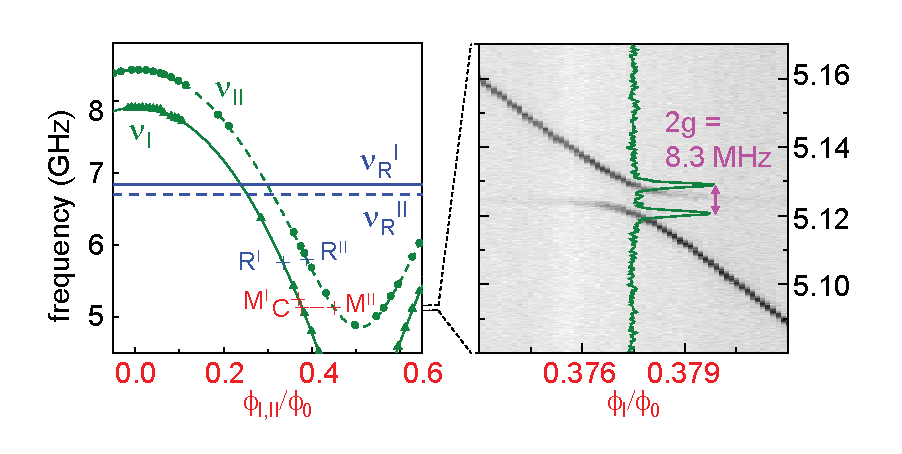
\includegraphics[width=0.8\textwidth]{./material/papers/iswap/figures/2_qubit_processor_spectrocopy}
	\label{fig:ProcessorSpectroscopy}
	\caption{}
\end{figure}

\subsection{Requirements}

%-List requirements for diVincenzo-style quantum computation:
%-Good 1 & 2 Qubit Gates
%-Qubits can be reset
%-Individual Single Shot Readout with High Fidelity

\subsection{Design \& Implementation}

%-Discuss the design & realization of our 2-qubit processor:
%  -Chip design
%  -Analytical model and parameter design.
%  -Measurement setup & RF chain

\section{Characterization of the Processor}

%-Show basic characteristics of the processor:
%  -Qubit transition energies vs. fluxes
%  -Qubit fast frequency controls
%  -2 Qubit interaction

\subsection{Readout}

%-Discuss the readout errors and crosstalk

\subsection{Single-Qubit Manipulation}

%-Discuss single qubit manipulation, gate fidelity and state tomography
%Data: 14/12/2010

\subsection{Implementing an Universal 2-Qubit Gate: $\sqrt{i\mathrm{SWAP}}$}

\begin{figure}
	\centering
		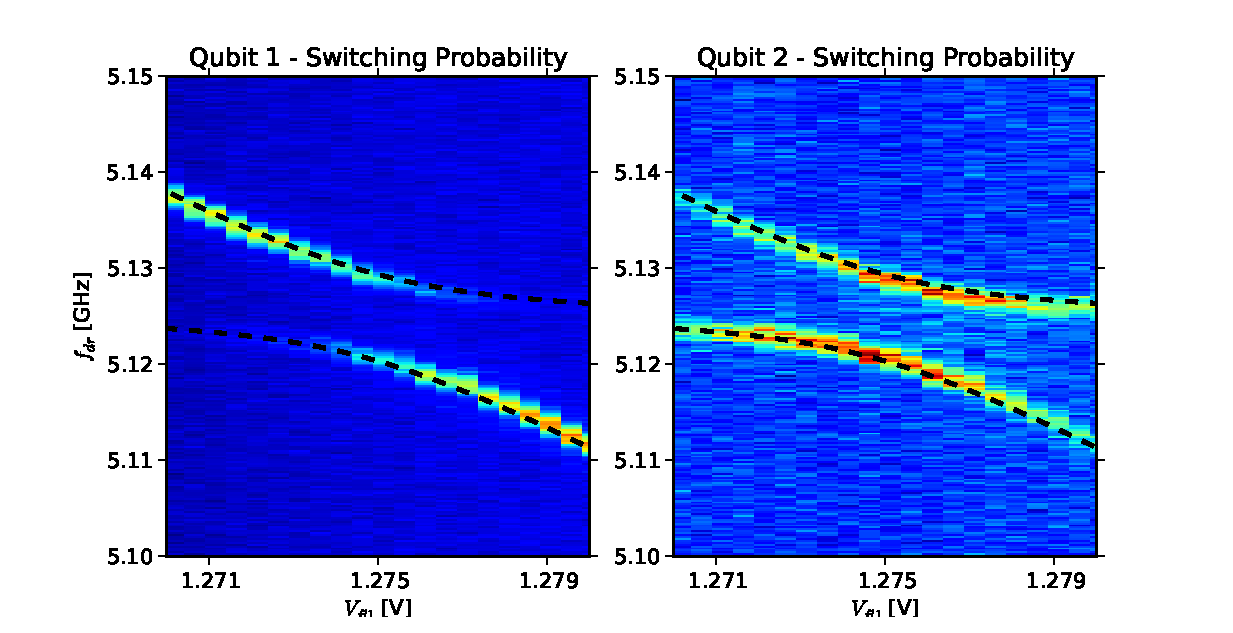
\includegraphics[width=1.\textwidth]{./material/figures/2-qubit-processor/characterization/anticrossing/anticrossing}
	\label{fig:QubitAnticrossing}
	\caption{}
\end{figure}


\begin{figure}
	\centering
		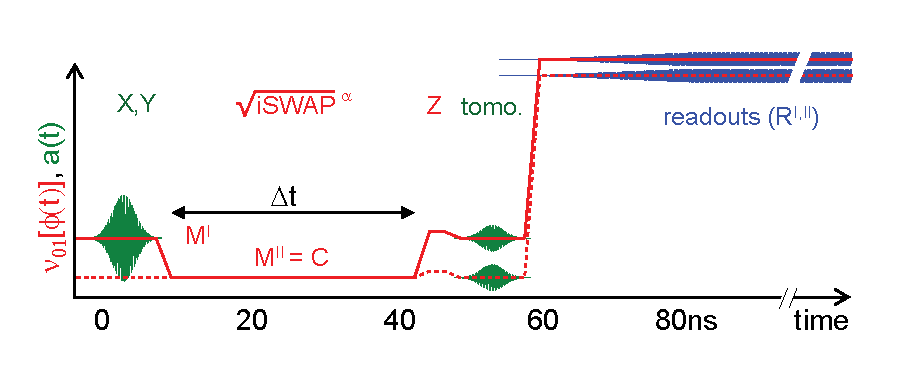
\includegraphics[width=0.8\textwidth]{./material/papers/iswap/figures/iswap_gate_pulse_sequence}
	\label{fig:ISwapPulseSequence}
	\caption{}
\end{figure}


%-Discuss the realization of a 2 qubit gate:
%  -Principle
%  -Implementation & Pulse Sequency
%  -Characterization through Quantum Process Tomography:
%     -Principles: State tomography, Pauli set, process tomography
%     -Discuss alternative representations of the process information:
%        -Chi matrix, Choi matrix, S, log S, Kraus operator representation
%  		-Errors: Discuss simulations, error models and possible reasons for discrepancies

%-Discuss the generation of Bell states, the measurement of entanglement witnesses and the measured violation of the CHSH equation.


%To Do:
% -Look through the swapping data and see if there's evidence for wavefunction collapse in qubit 2 when qubit 1 is measured and the two qubits are only partially entangled. Compare the Leo's proposition.

\subsection{Violation of Bell's inequality}

\begin{figure}
	\centering
		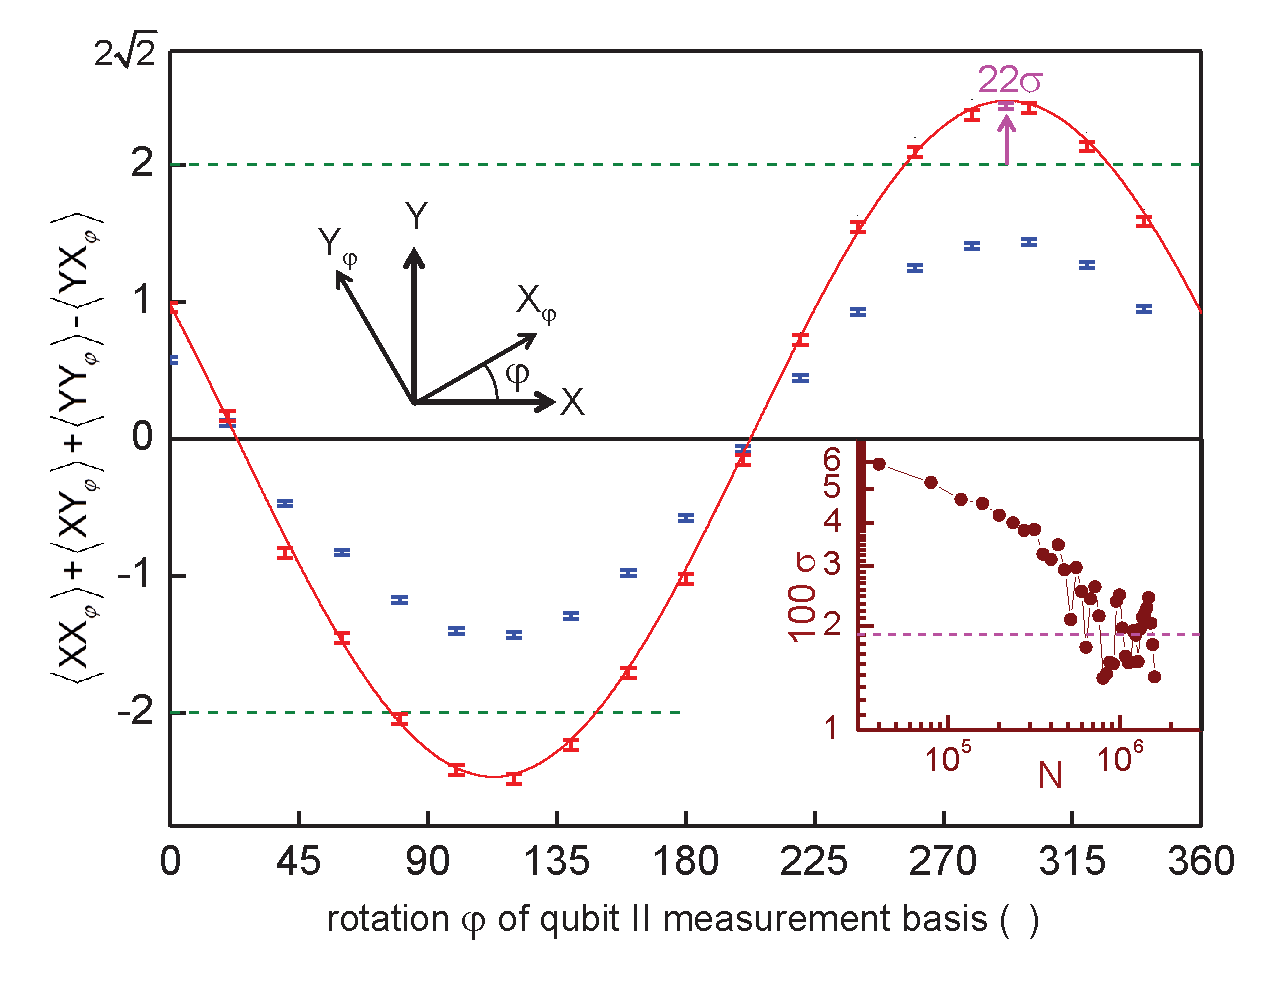
\includegraphics[width=0.8\textwidth]{./material/papers/iswap/figures/chsh}
	\label{fig:CHSH}
	\caption{}
\end{figure}

\subsection{Quantum State Tomography}

Quantum state tomography is the procedure of experimentally determining an unknown quantum state\cite{michael_a._nielsen_quantum_2000}.

\begin{eqnarray}
\rho & = & \sum\limits_{v_1,v_2\hdots v_n} \frac{c_{v_1,v_2\hdots v_n} \sigma_{v_1}\otimes \sigma_{v_2}\hdots \sigma_{v_n}}{2^n} \label{eq:state_tomography_state_representation} \\
c_{v_1,v_2\hdots v_n} & = & \mathrm{tr}\left(\sigma_{v_1}\otimes \sigma_{v_2}\hdots \sigma_{v_n} \; \rho \right)  \label{eq:state_tomography_coefficients}
\end{eqnarray}

where $v_i \in \left\{ X,Y,Z,I\right\}$ and $n$ gives the number of qubits in the system. To determine the coefficients $c_{v_1,v_2\hdots v_n}$ we prepare an ensemble of identical states $\rho$ and measure the expectation value of the operator $\sigma_{v_1}\otimes \sigma_{v_2}\hdots \sigma_{v_n}$. However, this would involve measuring the expectation values of the operators $\sigma_{X}$ and $\sigma_{Y}$, which we cannot do in experiment. Therefore, instead of directly measuring $\sigma_x$ or $\sigma_y$, we perform a rotation $\Theta_{\pi /2}(Y)$ or $\Theta_{-\pi /2}(X)$ first and measure $\sigma_z$ afterwards, which yields the same result. \todo{check the signs of the rotations!}

Repeating this method many times and averaging the result then gives an estimate of the coefficients $c_{v_1,v_2\hdots v_n}$. Unfortunately, when estimating these coefficients one-by-one, small measurement and preparation errors can yield a density matrix $\rho$ which is {\it non-physical} i.e. which violates the positivity or unity-trace properties of a physical density matrix. There, often we use techniques for jointly estimating all $c_{v_1,v_2\hdots v_n}$'s within the set of acceptable density matrices.

\subsubsection{Maximum Likelihood Estimation}

A method which is often used in quantum state tomography is the so-called {\it maximum-likelihood} technique, which works in the following way:

\subsection{Process Tomography of the Quantum Gate}

A quantum process can be described as a map $\mathcal{E} : \rho_\mathcal{H} \to \rho_\mathcal{H}$ that maps a density matrix $\rho$ defined in a Hilbert space $Q_1$ to another density matrix $\mathcal{E}(\rho)$ defined in a target Hilbert space $Q_2$ and fulfilling three axiomatic properties \cite{michael_a._nielsen_quantum_2000,haroche_exploring_2006}:

\begin{axiom}
$\mathrm{tr}\left[\mathcal{E}(\rho)\right]$ is the probability that the process represented by $\mathcal{E}$ occurs, when $\rho$ is the initial state.
\end{axiom}

\begin{axiom}
$\mathcal{E}$ is a {\it convex-linear map} on the set of density matrices, that is, for probabilities $\left\{p_i\right\}$,

  \begin{equation}
	  \mathcal{E}\left(\sum\limits_i p_i \rho_i\right) = \sum\limits_i p_i \mathcal{E}(\rho_i)
	\end{equation}
\end{axiom}

\begin{axiom}
$\mathcal{E}$ is a {\it completely-positive} map. That is, if $\mathcal{E}$  maps density operators of system $Q_1$ to density operators of system $Q_2$, then $\mathcal{E}(A)$ must be positive for any positive operator $A$. Furthermore, if we introduce an extra system $R$ of arbitrary dimensionality, it must be true that $(\mathcal{I}\otimes \mathcal{E})(A)$ is positive for any positive operator $A$ on the combined system $RQ_1$, where $\mathcal{I}$ denotes the identity map on system $R$.
\end{axiom}
As shown in \cite{michael_a._nielsen_quantum_2000}, any quantum process fulfilling these criteria can be written in the form

\begin{equation}
  \mathcal{E}(\rho) = \sum\limits_i E_i \rho E_i^\dagger \label{eq:process_operator_sum_representation}
\end{equation}
for some set of operators $\{ E_i \}$ which map the input Hilbert space to the output Hilbert space, and $\sum_i E_i^\dagger E_i \le I$.

Now, if we express the operators $E_i$ in a different operator basis $\tilde{E}_j$ such that $E_i = \sum_j a_{ij} \tilde{E}_{j}$ and insert into eq. (\ref{eq:process_operator_sum_representation}), we obtain

\begin{eqnarray}
 \mathcal{E}(\rho) & = & \sum\limits_i \sum\limits_j a_{ij} \tilde{E}_j \;\rho\; \sum\limits_k a_{ik}^* \tilde{E}_k^\dagger \\
& = & \sum\limits_{j,k}\tilde{E}_j \; \rho \; \tilde{E}_k^\dagger \sum\limits_i a_{ij} a_{ik}^* \\
& = & \sum\limits_{j,k}\tilde{E}_j \; \rho \; \tilde{E}_k^\dagger \; \chi_{jk} \label{eq:process_chi_representation}
\end{eqnarray}
where we defined $\chi_{jk} = \sum\limits_i a_{ij} a_{ik}^*$. This is the so-called $\chi$-matrix representation of the quantum process. Here, all the information on the process is contained in the $\chi$ matrix, which controls the action of the process-independent operators $\tilde{E}_i$ on the initial density matrix $\rho$.

Now, the goal of {\it quantum process tomography} is to obtain the coefficients of the $\chi$-matrix -- or any other complete representation of the process -- from a set of experimentally measured density matrices $\rho$ and $\mathcal{E}(\rho)$.

To achieve this, several techniques have been developed. The technique used in this work is the so-called {\it standard quantum process tomography (SQPT)}. This technique proceeds as follows:

\begin{enumerate}
\item Choose a set of operators $E_i$ that forms a full basis of $\mathcal{M}: Q_1 \to Q_2$. For n-qubit process tomography we usually choose $E_{i_1,i_2 \hdots i_n} = \sigma_{i_1}\otimes \sigma_{i_2}\hdots\otimes\sigma_{i_n}$, where $\sigma_i$ are the single-qubit Pauli operators and $i\in\{I,X,Y,Z\}$. 
\item Choose a set of pure quantum states $\ket{\phi_i}$ such that $\ket{\phi_i}\bra{\phi_i}$ span the whole space of input density matrices $\rho$. Usually, for a n-qubit system we choose $\phi = \{\ket{0},\ket{1},(\ket{0}+\ket{1})/\sqrt{2},(\ket{0}+i\ket{1})/\sqrt{2}\}^{\otimes n}$, where $^{\otimes n}$ denotes the n-dimensional Kronecker product of all possible permutations.
\item For each of the $\ket{\phi_i}$, determine $\mathcal{E}(\ket{\phi_i}\bra{\phi_i})$ by quantum state tomography. Usually we also determine $\ket{\phi_i}\bra{\phi_i}$ experimentally since the preparation of this state already entails small preparation errors that should be taken into account when performing quantum process tomography. 
\end{enumerate}

After having obtained the $\rho_i$ and $\mathcal{E}(\rho_i)$ one obtains the $\chi$-matrix by writing $\mathcal{E}(\rho_i) = \sum_j \lambda_{ij} \tilde{\rho}_j$, with some arbitrary basis $\tilde{\rho}_j$ and
letting $\tilde{E}_m \tilde{\rho}_j \tilde{E}_n^\dagger = \sum_k \beta_{jk}^{mn}\tilde{\rho}_k$. We can then insert into eq. (\ref{eq:process_chi_representation}) and obtain
\begin{eqnarray}
\sum\limits_k \lambda_{ik} \tilde{\rho}_k & = & \sum\limits_{m,n} \chi_{mn} \sum\limits_k \beta_{ik}^{mn} \tilde{\rho}_k  
\end{eqnarray}
This directly yields $\lambda_{ik} = \sum_{m,n}\beta_{ik}^{mn}\; \chi_{mn}$, which, by linear inversion,  gives $\chi$.

\subsubsection{The Kraus representation}

Besides the $\chi$-matrix representation, there is another useful way of expressing a quantum map, the so called {\it Kraus representation}, which is given as

\begin{equation}
 \mathcal{E}(\rho) = \sum\limits_i M_i \; \rho \; M_i^\dagger \label{eq:process_kraus_representation}
\end{equation}

It can be shown \citep{haroche_exploring_2006} that this sum contains at most $N$ elements, where $N$ is the dimension of the Hilbert space of the density matrix $\rho$. We can go from the $\chi$ representation to the Kraus representation by changing the basis $\tilde{E}_i$ such that

\begin{equation}
	\tilde{E}_i = \sum\limits_l a_{il}\; \breve{E}_l
\end{equation}

which, for eq. (\ref{eq:process_chi_representation}), yields

\begin{eqnarray}
 \mathcal{E}(\rho) & = & \sum\limits_{j,k} \sum\limits_l a_{jl} \breve{E}_l \; \rho \sum\limits_m a_{km}^* \breve{E}_m^\dagger \; \chi_{jk} \\
 & = & \sum\limits_{l,m}  \breve{E}_l \; \rho \; \breve{E}_m^\dagger \; \sum\limits_{j,k} a_{jl} a_{km}^* \chi_{jk} \label{eq:process_chi_transformed}
\end{eqnarray}

The last sum on the right side of eq. (\ref{eq:process_chi_transformed}) corresponds to a change of coordinates of the matrix $\chi$. Now, we can pick the $a$ such that $\chi$ is diagonal in the new basis $\breve{E}$ and obtain

\begin{eqnarray}
 \mathcal{E}(\rho) & = &  \sum\limits_{l} \lambda_l \breve{E}_l \; \rho \; \breve{E}_l^\dagger \\
& = &  \sum\limits_{l} M_l \; \rho \; M_l^\dagger
\end{eqnarray}
with $\lambda_l$ being the $l$-th eigenvalue of the $\chi$ matrix with the eigen-operator $\breve{E}_l$ and $M_{l} = \sqrt{\lambda_l} \breve{E}_l$.

\begin{figure}
	\centering
		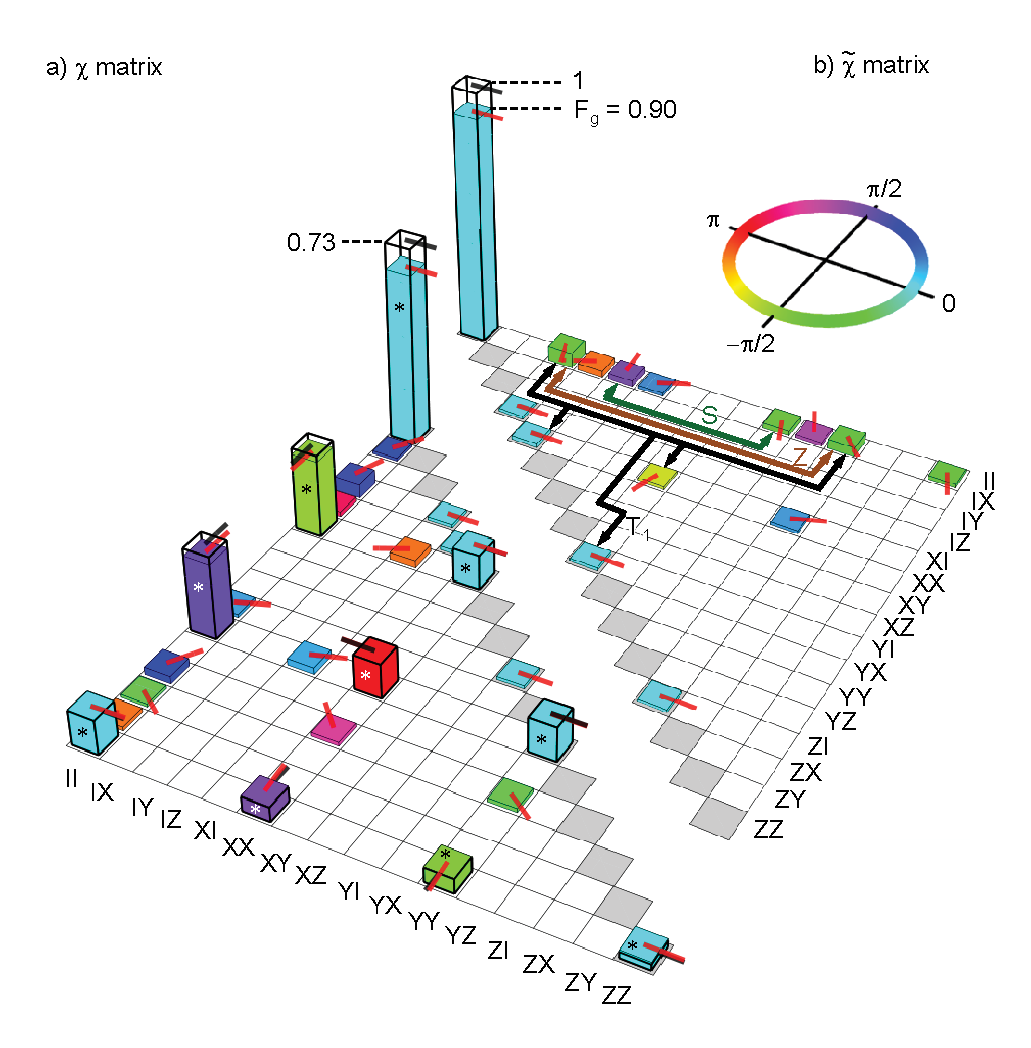
\includegraphics[width=1.\textwidth]{./material/papers/iswap/figures/chi_matrix_and_error_process}
	\label{fig:GateChiMatrixAndErrorProcess}
	\caption{}
\end{figure}


\section{Running Grover's Search Algorithm}

%Motivate this experiment:
% -Benchmark for superconducting quantum computers
% -Speed-up for searching in an unsorted database

\begin{figure}
	\centering
		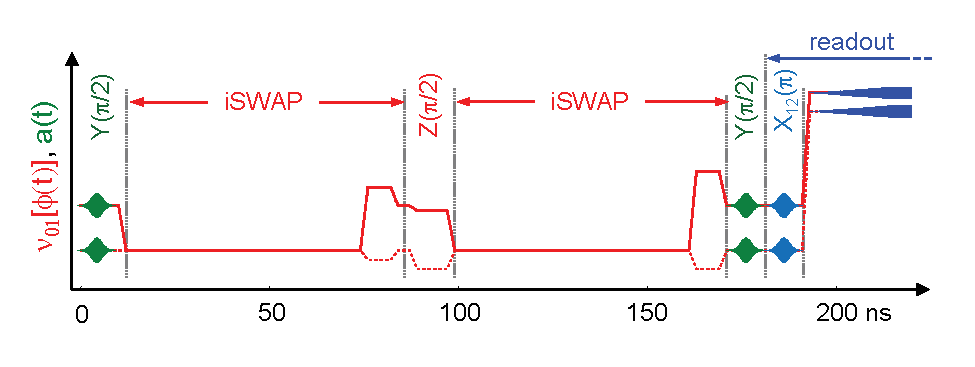
\includegraphics[width=1.\textwidth]{./material/papers/grover/figures/grover_algorithm_pulse_sequence}
	\label{fig:Grover3}
	\caption{The pulse sequence used in realizing Grover's quantum search algorithm. First, a $Y_{\pi/2}$ pulse is applied to each qubit to produce the fully superposed state $1/2(\ket{00}+\ket{01}+\ket{10}+\ket{11})$. Then, an $i\mathrm{SWAP}$ gate is applied, followed by a $Z_{\pm \pi /2}$ gate on each qubit, which corrsponds to the application of the oracle function. The resulting state is then analyzed using another $i\mathrm{SWAP}$ gate and two $Y_{\pi/2}$ gates to extract the state which has been marked by the oracle function. Optionally, a $Y^{12}_{\pi}$ pulse is used on each qubit to increase the readout fidelity.}
\end{figure}

\subsection{Introduction \& Motivation}

\begin{enumerate}
  \item {\textbf Inputs:} An oracle function $\mathcal{O}$ which performs the operation $O\ket{x}\ket{q} = \ket{x}\ket{q\otimes f(x)}$, where $f(x) = \delta_{x,x_0}$
  \item {\textbf Outputs:} The marked state $x_0$
	\item Initialize the qubit register to the state: 
	$$\ket{\psi} \to \ket{0}^{\otimes n}\ket{0}$$
	\item Apply the Hadamard transformation to all of the qubits: 
	$$\ket{psi}\to \frac{1}{\sqrt{2^n}}\sum\limits_{x=0}^{2^n-1} \ket{x} \left[ \frac{\ket{0}-\ket{1}}{\sqrt{2}} \right]$$
	\item Apply the Grover iteration $R \approx [\pi \sqrt{2^n}/4]$ times:
	$$ \ket{\psi} \to \left[(2 \ket{\psi}\bra{\psi}-I)\mathcal{O}\right]^R \frac{1}{\sqrt{2^n}} \sum\limits_{x=0}^{2^n-1}\ket{x} \left[ \frac{\ket{0}-\ket{1}}{\sqrt{2}} \right] \approx \ket{x_0}\left[\frac{\ket{0}-\ket{1}}{\sqrt{2}}\right] $$
	\item Measure the first n qubits to obtain $x_0$
\end{enumerate}

For the 2-qubit case, this algorithm can be drastically simplified -- or ``compiled'' -- such that it runs without the ancilla qubit and in one single step of the Grover iteration:

\begin{enumerate}
  \item {\textbf Inputs:} An oracle function $\mathcal{O}$ which performs the operation $O\ket{x} =(-1)^{\delta_{x,x_0}}\ket{x}$, where $x_0$ is the marked state that is searched.
  \item {\textbf Outputs:} The marked state $x_0$
	\item 
\end{enumerate}

%-Explain the Grover experiment...
%		-Theoretical interest
%		-First demonstration in NMR
%   -Potential speed-up
%   -Details of the algorithm:
%     -Elementary operations
%     -Pulse shapes, corrections, ...

\begin{figure}
	\centering
		\includegraphics[width=1.\textwidth]{./material/papers/grover/figures/grover_algorithm_schematic}
	\label{fig:GroverAlgorithmSchematic}
	\caption{}
\end{figure}

\subsection{Experimental Implementation}

%-Show the implementation principle of the experiment.
%  -Break down the algorithm using the universal quantum gates that we've implemented

\subsection{Results}

%To Do:
%  -Create figures for all steps of the algorithm using Matplotlib
%  -Re-Analyze the data using Denis' Mathematica
%-Discuss the results and errors.

\begin{figure}
	\centering
		\includegraphics[width=1.\textwidth]{./material/papers/grover/figures/grover_algorithm_experimental_results}
	\label{fig:GroverAlgorithmExperimentalResults}
	\caption{}
\end{figure}

\subsection{Conclusions}

%-Conclusions regarding quantum speed-up and applicability of results to larger-scale quantum computing.


\input{"scalable architecture"}

\chapter{Perspective \& Future Directions}

In chapters \ref{chapter:processor_characterization} and \ref{chapter:grover_algorithm} we demonstrated a universal two-qubit gate on our quantum processor and used it to realize the two-qubit Grover search algorithm, achieving probabilistic quantum speed-up. However, this approach to quantum computing cannot be scaled beyond a few qubits, wich is mostly due to the nature of the qubit-qubit coupling that has been chosen: The direct capacitive coupling produces a qubit-qubit interaction which is always on and whose amplitude decreases as $g_{qq}/\Delta_{qq}$. To be able to realize gate times which are shorter than the typical coherence time of Transmon qubits (typically $T_1,T_\phi \simeq\ 1-10 \;\mathrm{\mu s}$) we require coupling strengts $g_{qq}/2\pi \ge 10\;\mathrm{MHz}$. Therefore, in order to switch of spurious coupling between any two qubits below the 5 \% level, a detuning of $\Delta_{qq}\ge 20g \simeq 200\;\mathrm{MHz}$. For a processor where one would couple a large number of qubits using this scheme, the required qubit-qubit detunings would quickly lead to so-called {\it frequency crowding}, i.e. a shortage of available working point frequencies for the different qubits of the processor.

\smallskip

Hence, for a larger-scale quantum processor, it is essential to devise a coupling scheme which allows to deterministically turn on and off the coupling between arbitary qubits. In the literature, several architectures have been proposed for this, using e.g. a parametric coupling between qubits \citep{bertet_parametric_2006} or relying on the storage of quantum information stored in the qubits in a seperate entity, such as a superconducting resonator \citep{galiautdinov_resonatorzero-qubit_2012,mariantoni_implementing_2011}.

\smallskip

In the following section, we will propose a different approach to scalable quantum computing, based on a recently introduced double Transmon qubit \citep{srinivasan_tunable_2011} and using a fixed-frequency, microwave-tunable qubit-qubit coupling scheme as well as a single-shot readout method for individual qubits.

\smallskip

After shortly discussing our proposed architecture, we discuss recent developments in superconducting quantum computing and put them in context with our work, indicating possible future research directions.

\section{Designing a Scalable Architecture for Quantum Bits} \label{section:scalable_architecture}

In this section we describe our proposal for a scalable multi-qubit architecture based on superconducting Transmon qubits and fulfilling all of DiVincenzo's criteria for the realization of a quantum computer, as discussed in section \ref{section:divincenzo_criteria}. \citep{steane_how_2007}

\subsection{Requirements}

A scalable architecture for quantum computing should fulfill all criteria discussed above and, in addition do not incur an exponential experimental overhead for each qubit that is added to the quantum computer \citep{blume-kohout_climbing_2002}. Today, the two issues that are not addressed well by current qubit architectures, such as the quantum bus architecture used by many groups today \citep{dicarlo_demonstration_2009,wallraff_strong_2004}, which concern the qubit-qubit coupling and the readout of individual qubits. The quantum bus architecture, for instance, has an always-on coupling scheme between the qubits described by eq. (\ref{eq:cqed_bus_coupling}) which makes it hard to precisely control the coupling between individual qubits if a large number of them is present. Also, the readout of the qubit register is usually performed as a joint readout of the whole qubit register, thereby not allowing the read out of individual qubits.

\subsection{Qubit Parameters}

\begin{SCfigure}[1.0][ht!]
	\centering
	\includegraphics[width=0.35\textwidth]{./material/figures/scalable-architecture/qubit_molecule}
	\caption[...]{...}
	\label{fig:qubit_molecule_energies}
\end{SCfigure}

%
\begin{eqnarray}
\hat{H}_{dt}       & = & \hat{H}_q+\hat{H}_{qq} \\
\hat{H}_{q}/\hbar  & = & \omega_{01}^I\hat{\sigma}_z^I+\omega_{01}^{II}\hat{\sigma}_z^{II} \\
\hat{H}_{qq}/\hbar & = & g_{qq}\left(\hat{\sigma}_+^I\hat{\sigma}_-^{II}+\hat{\sigma}_-^I\hat{\sigma}_+^{II}\right) \\
\end{eqnarray}
%
We can rewrite $\hat{H}_{qq}$ in the eigenbasis $\ket{00}$, $\ket{01}$, $\ket{10}$, $\ket{11}$ of $\hat{H}_q$ as
%
\begin{equation}
\hat{H}_{qq}/\hbar = g_{qq}\left(\ket{10}\bra{01}+\ket{01}\bra{10}\right)
\end{equation}
%
When taking into account the second Transmon level $\ket{2}$, the capacitive coupling induces additional coupling elements
%
\begin{eqnarray}
\hat{H}_{qq}'/\hbar g_{qq} &  = &  \left(\ket{10}\bra{01}+\ket{01}\bra{10}\right) \\
& + & \sqrt{2}\left(\ket{11}\bra{02}+\ket{02}\bra{11}\right) \\
& + & \sqrt{2}\left(\ket{11}\bra{20}+\ket{20}\ket{11}\right) \\
& + & 2\left(\ket{21}\bra{12}+\ket{12}\bra{21}\right)
\end{eqnarray}
%
\subsection{Qubit-Qubit Coupling}

We couple the double Transmon to the resonator as shown in fig. \ref{fig:double_transmon_schematic} such that each of the two Transmons couples to the resonator with the same constant $g_{01}$. The resulting Hamiltonian, in analogy to Hamiltonian (\ref{eq:cqed_bus_coupling}) is
%
\begin{equation}
\hat{H}_{qr}/\hbar = g_{01}^I\left(\hat{\sigma}_+^I\hat{a}+\hat{\sigma}_-^I\hat{a}^\dagger\right)+g_{01}^{II}\left(\hat{\sigma}_+^{II}\hat{a}+\hat{\sigma}_-^{II}\hat{a}^\dagger \right), \label{eq:double_transmon_resonator_coupling}
\end{equation}
%
where, as before, the Hamiltonian of the resonator is given by eq. (\ref{eq:lc_hamiltonian}). As can be seen, the coupling operator between the two qubits and the resonator contains the sums $\hat{\sigma}_+^{I+II}=\hat{\sigma}_+^I+\hat{\sigma}_-^{II}$ and $\hat{\sigma}_-^{I+II}=\hat{\sigma}_-^I+\hat{\sigma}_-^{II}$. The eigenstates of $\hat{H}_{dt}$ at resonance $\omega_{01}^I)\omega_{01}^{II}$ are given as $\ket{00}$,$\ket{11}$, $\ket{\psi_+}=1/\sqrt{2}(\ket{01}+\ket{10})$ and $\ket{\psi_-}=1/\sqrt{2}(\ket{01}-\ket{10})$. Writing the Hamiltonian (\ref{eq:double_transmon_resonator_coupling}) in this eigenbasis yields
%
\begin{equation}
\hat{H}_{qr} = \sqrt{2}g_{01}\left[\left(\ket{11}\bra{\psi_+}+\ket{\psi_+}\bra{00}\right)\hat{a}+\left(\ket{\psi_+}\bra{11}+\ket{00}\bra{\psi_+}\right)\hat{a}^\dagger\right].
\end{equation}
%
As can be seen, the state $\ket{\psi_-}$ does not couple at all to the resonator, whereas the state $\ket{\psi_+}$ couples to it with an enhanced coupling rate $\sqrt{2}g_{01}$. The states $\ket{01}=(\ket{\psi_+}+\ket{\psi_-})/sqrt{2}$ and $\ket{10}=(\ket{\psi_+}-\ket{\psi_-})/\sqrt{2}$ couple to it at the normal rate $g_{01}$. Thus, if we operate the double Transmon at $\omega_{01}^I=\omega_{01}^{II}$ and ``park'' the qubit in the state $\ket{\psi_-}$, we can effectively switch off the coupling to the resonator. As proposed in \citep{srinivasan_tunable_2011}, we can peform an adiabatic passage $\ket{\psi_-}\to\ket{10}$ to switch on the qubit-resonator coupling of two or more qubits and perform a multi-qubit gate. Going back to the parking state $\ket{\psi_-}$ turns off the coupling again.

\subsection{Designing A Four-Qubit Architecture}

\begin{figure}[ht!]
	\centering
	\includegraphics[width=\textwidth]{./material/figures/scalable-architecture/qubit_architecture_energy_levels}
	\caption[]{}
	\label{fig:scalable_architecture_energy_levels}
\end{figure}

\subsection{Implementation}

\begin{figure}[ht!]
	\centering
	\includegraphics[width=\textwidth]{./material/figures/scalable-architecture/scalable_architecture_photos}
	\caption[]{}
	\label{fig:scalable_architecture_photos}
\end{figure}

\subsection{Scaling Up}

\section{Future Directions in Superconducting QC}

%-Discuss further developments in superconducting qc, such as:

\subsection{3D Circuit Quantum Electrodynamics}

%-Discuss the significance and potential of Q3CED

\subsection{Hybrid Quantum Systems}

%-Discuss hybrid quantum systems such as NV centers and their potential.
%  -Yui's & NTT NV center experiments
%  -Problems and possible solutions

\subsection{Quantum Error Correction \& Feedback}

%-Discuss quantum error correction.
%-Discuss quantum feedback.
%  -Siddiqi experiment, Yale paper
%  -Future directions taking into account the availability of highly coherent Transmon qubits


\appendix

\input{"appendix - modeling"}

\input{"appendix - data acquisition"}

\input{"appendix - fabrication"}

\bibliographystyle{apalike}

\stepcounter{chapter}

\addcontentsline{toc}{chapter}{\numberline {\thechapter} Bibliography}

\bibliography{thesis}

\end{document}
